\documentclass[a4paper]{book}

\usepackage{geometry}
\usepackage{amsmath}
\usepackage{amssymb}
\usepackage{amsthm}
% \usepackage{newpxtext}
% \usepackage{newpxmath}
\usepackage[shortlabels]{enumitem}
\usepackage{tikz}
\usepackage{tikz-cd}
\usepackage{float}
\usepackage[colorlinks]{hyperref}
\usepackage{fixdif}

\allowdisplaybreaks[4]

\bibliographystyle{alpha}

\theoremstyle{definition}
\newtheorem{defn}{Definition}[section]
\newtheorem{eg}[defn]{Example}
\newtheorem{cons}[defn]{Construction}
\newtheorem{sym}[defn]{Notation}
\theoremstyle{plain}
\newtheorem{thm}[defn]{Theorem}
\newtheorem{prop}[defn]{Proposition}
\newtheorem{cor}[defn]{Corollary}
\newtheorem{lem}[defn]{Lemma}
\theoremstyle{remark}
\newtheorem{rem}[defn]{Remark}

\DeclareMathOperator{\sgn}{sgn}
\DeclareMathOperator{\Bl}{Bl}
\DeclareMathOperator{\res}{res}
\DeclareMathOperator{\im}{im}
\DeclareMathOperator{\coker}{coker}
\DeclareMathOperator{\preim}{preim}
\DeclareMathOperator{\Pic}{Pic}

\numberwithin{equation}{section}

\tikzset{every picture/.style={line width=0.7pt}}

\title{A Note on Complex Manifolds}
\author{Zeng Mengchen}
\date{Last compile: \today}

\begin{document}

\maketitle
\thispagestyle{empty}

\frontmatter

\tableofcontents
\newpage
\thispagestyle{empty}

\chapter{Preface}

This is a lecture note of a seminar on complex manifolds, by OM Society of School of Mathematical Scieces, Beijing Normal University.
We mainly follow \textsc{Kodaira} and \textsc{Morrow}'s classic~\cite{Kodaira06} and \textsc{Kodaira}'s later work~\cite{Kodaira05}.
We shall cover the part of complex manifolds, sheaf cohomology and geometry of complex manifolds.
Deformation theory will be skipped.
Numbering of sections will not follow the textbook, but for some important theorems we shall give the name or original numbering on the textbook.

This note is unfinished and will update continuously, it will be post on GitHub.
The repository name is \href{https://github.com/matthewzenm/complex-manifolds-seminar}{matthewzenm/complex-manifolds-seminar}.
Many typos and grammar mistakes will occur in this note, since I'm writing on my local machine and without spell checker.
If you find some typos or grammar mistakes, please contact me so that I can fix them.

\begin{flushright}
    Mengchen M.\ Zeng

    Aug 24, 2023
\end{flushright}

\newpage
\thispagestyle{empty}

\mainmatter

\chapter{Complex Manifolds}

In this chapter we introduce the elements of several complex variables and the notion of complex manifolds.
We also provide some examples of complex ma\-nifolds.

\section{Holomorphic maps}

\begin{defn}
    A complex valued function $f(z)$ on a connected open subset $W\subset\mathbb{C}^n$ is called \emph{holomorphic}, if for each $a=(a_1,\cdots,a_n)\in W$, $f(z)$ can be expanded as a convergent power series
    \[f(z)=\sum_{k_1\geq 0,\cdots,k_n\geq 0}c_{k_1\cdots k_n}(z_1-a_1)^{k_1}\cdots(z_n-a_n)^{k_n}\]
    in some neighborhood of $a$.
\end{defn}

From now on we shall use \emph{domain} to denote a connected open set.

\begin{prop}
    If $p(z)=\sum c_{k_1\cdots k_n}(z_1-a_1)^{k_1}\cdots(z_n-a_n)^{k_n}$ converges at $z=w$, then $p(z)$ converges for every $z$ with $|z_k-a_k|<|w_k-a_k|,\ k=1,\cdots,n$.
\end{prop}
\begin{proof}
    Left to reader.
\end{proof}

\begin{defn}
    The neighborhood above is called a \emph{polydisc} or \emph{polycylinder}, and denoted by $P(a,r)=\{z\in\mathbb{C}^n:\ |z_k-a_k|<r_k,\ k=1,2,\cdots,n\}$.
\end{defn}

A complex valued function of $n$ complex variables can be seen as a function of $2n$ real variables, thus we have the following definition.
\begin{defn}
    A complex valued function of $n$ complex variables is \emph{continuous} or \emph{differentiable}, if it is continuous or differentiable as a function of $2n$ real variables.
\end{defn}

We have

\begin{thm}[Osgood]\label{osgood}
    Let $f(z_1,\cdots,z_n)$ be a continuous function on the domain $W\subset\mathbb{C}^n$, if $f$ is holomorphic with respected to each $z_k$ and other $z_i$'s fixed, then $f$ is holomorphic on $W$.
\end{thm}
\begin{proof}
    Let $a\in W$ lie in the polydisc $\overline{P(a,r)}\subset W$, we use Cauchy's integral formula iteratively:
    \begin{gather*}
        f(z_1,z_2,\cdots,z_n)=\frac{1}{2\pi\sqrt{-1}}\int_{|z_1-a_1|=r_1}\frac{f(w_1,z_2,\cdots,z_n)}{w_1-z_1}\d{w_1}\\
        f(w_1,z_2,\cdots,z_n)=\frac{1}{2\pi\sqrt{-1}}\int_{|z_2-a_2|=r_2}\frac{f(w_1,w_2,\cdots,z_n)}{w_2-z_2}\d{w_2}\\
        \cdots
    \end{gather*}
    Substituting, we have
    \[\left(\frac{1}{2\pi\sqrt{-1}}\right)^n\idotsint_{\partial P(a,r)}\frac{f(w_1,\cdots,w_n)}{(w_1-z_1)\cdots(w_n-z_n)}\d{w_1}\cdots\d{w_n}\]
    Since
    \[\left|\frac{z_k-a_k}{w_k-a_k}\right|<1\]
    The series
    \begin{align*}
        \frac{1}{w_k-z_k}&=\frac{1}{(w_k-a_k)-(z_k-a_k)}=\frac{1}{w_k-a_k}\cdot\frac{1}{1-(z_k-a_k)/(w_k-a_k)}\\
        &=\frac{1}{w_k-a_k}\sum_{i=0}^\infty\left(\frac{z_k-a_k}{w_k-a_k}\right)^i
    \end{align*}
    converges absolutely in $P(a,r)$, hence integrate term by term we have
    \[f(z_1,\cdots,z_n)=\sum_{k_0\geq 0,\cdots,k_n\geq 0}c_{k_1\cdots k_n}(z_1-a_1)^{k_1}\cdots(z_n-a_n)^{k_n}\]
    where
    \[c_{k_1\cdots k_n}=\left(\frac{1}{2\pi\sqrt{-1}}\right)^{k_1+\cdots+k_n}\idotsint_{\partial P(a,r)}\frac{f(w_1,\cdots,w_n)\d{w_1}\cdots\d{w_n}}{(w_1-a_1)^{k_1+1}\cdots(w_n-a_n)^{k_n+1}}\]
    Let $|f|\leq M$ on $\overline{P(a,r)}$, then we have
    \[|c_{k_0\cdots k_n}|\leq\frac{M}{r_1^{k_1}\cdots r_n^{k_n}}\]
    and for $z\in P(a,r)$, we have $|(z_k-a_k)/r_k|<1$, then
    \begin{align*}
        \left|\sum c_{k_1\cdots k_n}(z_1-a_1)^{k_1}\cdots(z_n-a_n)^{k_n}\right|&\leq M\left|\sum\left(\frac{z_1-a_1}{r_1}\right)^{k_1}\cdots\left(\frac{z_n-a_n}{r_n}\right)^{k_n}\right|\\
        &=M\prod_{k=1}^n\left|\frac{1}{1-(z_k-a_k)/r_k}\right|
    \end{align*}
    This shows the expansion is convergent for $z\in P(a,r)$.
    Since $a$ is arbitrary, $f$ is holomorphic.
\end{proof}

We now introduce the Cauchy--Riemann equations.

\begin{sym}
    Let $f$ be a differentiable function on a domain $W\subset\mathbb{C}^n$, denote
    \begin{gather}
        \frac{\partial}{\partial z_k}=\frac{1}{2}\left(\frac{\partial}{\partial x_k}-\sqrt{-1}\frac{\partial}{\partial y_k}\right)\\
        \frac{\partial}{\partial\overline{z_k}}=\frac{1}{2}\left(\frac{\partial}{\partial x_k}+\sqrt{-1}\frac{\partial}{\partial y_k}\right)
    \end{gather}
    for $z_k=x_k+\sqrt{-1}y_k$ and $1\leq k\leq n$.
\end{sym}

\begin{thm}
    Let $f$ be a (continuously) differentiable function on the domain $W\subset\mathbb{C}^n$, then $f$ is holomorphic on $W$ if and only if $\partial{f}/\partial{\overline{z_k}}=0$ for $k=1,\cdots,n$.
\end{thm}
\begin{proof}
    This is a corollary of Theorem~\ref{osgood} and classical results in complex analysis in one variable.
\end{proof}

\begin{prop}[Chain rule]
    Suppose $f(w_1,\cdots,w_m)$ and $g_k(z),\ k=1,\cdots,m$ are differentiable, and the domain of $f$ contains the range of $g=(g_1,\cdots,g_m)$, then $f\circ g$ is differentiable, and if $w_m=g_m(z)$, then
    \begin{gather*}
        \frac{\partial f(g(z)))}{\partial z_k}=\sum_{i=1}^m\left(\frac{\partial f(w)}{\partial w_i}\cdot\frac{\partial w_i}{\partial z_k}+\frac{\partial f(w)}{\partial\overline{w_i}}\cdot\frac{\partial\overline{w_i}}{\partial z_k}\right)\\
        \frac{\partial f(g(z)))}{\partial\overline{z_k}}=\sum_{i=1}^m\left(\frac{\partial f(w)}{\partial w_i}\cdot\frac{\partial w_i}{\partial\overline{z_k}}+\frac{\partial f(w)}{\partial\overline{w_i}}\cdot\frac{\partial\overline{w_i}}{\partial\overline{z_k}}\right)
    \end{gather*}
\end{prop}
\begin{proof}
    Direct calculation verifies the proposition.
\end{proof}

\begin{cor}
    If $f(w)$ is holomorphic in $w=(w_1,\cdots,w_m)$ and $g_k(z),\ k=1,\cdots,m$ are holomorphic in $z$, then $f\circ g$ is holomorphic in $z$.
\end{cor}

\begin{cor}
    The set $\mathcal{O}_{\mathbb{C}^n}(\Omega)$ of holomorphic functions on open set $\Omega$ forms a ring. (We use sheaf notation before we introduce what is a sheaf.)
\end{cor}

\begin{defn}
    A map $f(z)=(f_1(z),\cdots,f_m(z))$ from $\mathbb{C}^n$ to $\mathbb{C}^m$ is a \emph{holomorphic map} if each $f_k(z)$ is holomorphic, $k=1,\cdots,m$.
    The matrix
    \[\begin{bmatrix}
        \partial{f_1}/\partial{z_1} & \cdots & \partial{f_m}/\partial{z_1}\\
        \vdots & \ddots & \vdots \\
        \partial{f_1}/\partial{z_n} & \cdots & \partial{f_m}/\partial{z_n}
    \end{bmatrix}=:\left[\frac{\partial{f_i}}{\partial{z_j}}\right]_{1\leq i\leq m,1\leq j\leq n}\]
    is called \emph{Jacobian matrix}, and if $m=n$, the determinant $\det[\partial{f_i}/\partial{z_j}]$ is called the \emph{Jacobian}.
\end{defn}

Writing out $f_i=u_i+\sqrt{-1}v_i$ and $z_j=x_j+\sqrt{-1}y_j$, we denote briefly
\[\frac{\partial(u,v)}{\partial(x,y)}:=\det\left(\frac{\partial(u_1,v_1,\cdots,u_n,v_n)}{\partial(x_1,y_1,\cdots,x_n,y_n)}\right)\]
And we have
\begin{lem}\label{real jacobian}
    If $f$ is holomorphic, then $\partial(u,v)/\partial(x,y)=|\det[\partial{f_i}/\partial{z_j}]|^2\geq 0$.
\end{lem}
\begin{proof}
    Let
    \begin{gather*}
        \begin{bmatrix}
            \partial/\partial{z_1} & \partial/\partial{\overline{z_1}} & \cdots & \partial/\partial{z_n} & \partial/\partial{\overline{z_n}}
        \end{bmatrix}=A\\
        \begin{bmatrix}
            \partial/\partial{x_1} & \partial/\partial{y_1} & \cdots & \partial/\partial{x_n} & \partial/\partial{y_n}
        \end{bmatrix}=B
    \end{gather*}
    Then
    \[A=B\begin{bmatrix}
        1/2 & 1/2 & & & \\
        -\sqrt{-1}/2 & \sqrt{-1}/2 & & & \\
         & & 1/2 & 1/2 & \\
         & & -\sqrt{-1}/2 & \sqrt{-1}/2 & \\
         & & & & \ddots
    \end{bmatrix}\]
    Hence
    \begin{align*}
        \frac{\partial(u,v)}{\partial(x,y)}&=\det\begin{bmatrix}
            u_1 \\ v_1 \\ \vdots \\ u_n \\ v_n
        \end{bmatrix}\begin{bmatrix}
            \partial/\partial{x_1} & \partial/\partial{y_1} & \cdots & \partial/\partial{x_n} & \partial/\partial{y_n}
        \end{bmatrix}\\
        &=\left(\frac{\sqrt{-1}}{2}\right)^n\det\begin{bmatrix}
            u_1 \\ v_1 \\ \vdots \\ u_n \\ v_n
        \end{bmatrix}\begin{bmatrix}
            \partial/\partial{z_1} & \partial/\partial{\overline{z_1}} & \cdots & \partial/\partial{z_n} & \partial/\partial{\overline{z_n}}
        \end{bmatrix}\\
        &=\left(\frac{\sqrt{-1}}{2}\right)^n\det\begin{bmatrix}
            \partial{u_1}/\partial{z_1} & \partial{u_1}/\partial{\overline{z_1}} & \cdots & \partial{u_1}/\partial{z_n} & \partial{u_1}/\partial{\overline{z_n}}\\
            \partial{v_1}/\partial{z_1} & \partial{v_1}/\partial{\overline{z_1}} & \cdots & \partial{v_1}/\partial{z_n} & \partial{v_1}/\partial{\overline{z_n}}\\
            \vdots & \vdots & \ddots & \vdots & \vdots \\
            \partial{u_n}/\partial{z_1} & \partial{u_n}/\partial{\overline{z_1}} & \cdots & \partial{u_n}/\partial{z_n} & \partial{u_n}/\partial{\overline{z_n}}\\
            \partial{v_n}/\partial{z_1} & \partial{v_n}/\partial{\overline{z_1}} & \cdots & \partial{v_n}/\partial{z_n} & \partial{v_n}/\partial{\overline{z_n}}
        \end{bmatrix}
    \end{align*}
    Multiply $\sqrt{-1}$ on even rows, $1/2$ on odd rows, and add $2k$th row to ($2k-1$)st row, subtract ($2k-1$)st row to $2k$th row, we obtain
    \[\frac{\partial(u,v)}{\partial(x,y)}=\det\begin{bmatrix}
        \partial{f_1}/\partial{z_1} & & \cdots & \partial{f_1}/\partial{z_n} & \\
         & \overline{\partial{f_1}/\partial{z_1}} & \cdots & & \overline{\partial{f_1}/\partial{z_n}} \\
        \vdots & \vdots & \ddots & \vdots & \vdots \\
        \partial{f_n}/\partial{z_1} & & \cdots & \partial{f_n}/\partial{z_n} & \\
        & \overline{\partial{f_n}/\partial{z_1}} & \cdots & & \overline{\partial{f_n}/\partial{z_n}}
    \end{bmatrix}\]
    We expand the determinant, extract odd rows and even rows respectively, and we get
    \begin{align*}
        \frac{\partial(u,v)}{\partial(x,y)}&=\sum_{\sigma,\tau\in S_n}\sgn\sigma\sgn\tau\left(\frac{\partial{f_1}}{\partial{z_{\sigma(1)}}}\cdots\frac{\partial{f_n}}{\partial{z_{\sigma(n)}}}\right)\left(\overline{\frac{\partial{f_1}}{\partial{z_{\tau(1)}}}}\cdots\overline{\frac{\partial{f_n}}{\partial{z_{\tau(n)}}}}\right)\\
        &=\det[\partial{f_i}/\partial{z_j}]\overline{\det[\partial{f_i}/\partial{z_j}]}\\
        &=|\det[\partial{f_i}/\partial{z_j}]|^2\qedhere
    \end{align*}
\end{proof}

\begin{thm}[Inverse function theorem]
    Let $U\subset\mathbb{C}^n$ open, $f:U\to\mathbb{C}^n$ be a holomorphic map, $a\in U$.
    If $\det[\partial{f_i}/\partial{z_j}]_{z=a}\neq 0$, then for a sufficiently small neighborhood $N$ of $a$, $f$ is bijective on $N$, $f(N)$ is open and $f^{-1}|_{f(N)}$ is holomorphic on $f(N)$.
\end{thm}
\begin{proof}
    By Lemma~\ref{real jacobian}, $\partial(u,v)/\partial(x,y)\neq 0$ at $a$, then by the inverse function theorem of real functions, $f$ is bijective and differentiable, and $f(N)$ is open.
    We check that $f^{-1}|_{f(N)}$ is holomorphic.
    Set $\varphi(w)=f^{-1}(w)$, then $z_i=\varphi_i(f(z))$.
    Differentiate the equality gives
    \begin{align*}
        0=\frac{\partial z_i}{\partial\overline{z_k}}&=\sum_{j=1}^n\left(\frac{\partial\varphi_i(w)}{\partial w_j}\cdot\frac{\partial f_j(z)}{\partial\overline{z_k}}+\frac{\partial\varphi_i(w)}{\partial\overline{w_j}}\cdot\frac{\partial\overline{f_j(z)}}{\partial\overline{z_k}}\right)\\
        &=\sum_{j=1}^n\frac{\partial\varphi_i(w)}{\partial\overline{w_j}}\cdot\frac{\partial\overline{f_j(z)}}{\partial\overline{z_k}}
    \end{align*}
    Since $\det[\partial\overline{f_j(z)}/\partial\overline{z_k}]=\overline{\det[\partial f_j(z)/z_k]}\neq 0$, by linear algebra we have $\partial\varphi_i(w)/\partial\overline{w_j}=0$ for each $i,j$, that is, $\varphi$ is holomorphic.
\end{proof}

\section{Complex Manifolds}

\begin{defn}
    Let $M$ be a topological manifold.
    A \emph{coordinate chart} is an open set $U\subset M$ and a continuous map $\varphi:U\to\mathbb{C}^n$ that maps $U$ homeomorphically onto an open set of $\mathbb{C}^n$.
    An \emph{atlas} is a collection $\{(U_i,\varphi_i)\}_{i\in I}$ of coordinate charts that $M=\bigcup_{i\in I}U_i$ and for any $U_i\cap U_j\neq\varnothing$, $\varphi_i\circ\varphi_j^{-1}$ and $\varphi_j\circ\varphi_i^{-1}$ are both holomorphic.
    A \emph{complex structure} is a maximal atlas.

    A \emph{complex manifold} is a topological manifolds endowed with a complex structure.
\end{defn}

\begin{lem}
    Every complex manifold is paracompact, i.e.\ every open cover has a locally finite open refinement.
\end{lem}
\begin{proof}
    \cite[Theorem~4.77]{LeeTop}.
\end{proof}

In the rest of the section, we provide some examples and constructions of complex manifolds.

\begin{cons}
    The \emph{complex projective space} $\mathbb{P}^n$ is defined as the set of all $1$-dimensional subspaces of $\mathbb{C}^{n+1}$.
    It can be realized as the sphere $\{z\in\mathbb{C}^{n+1}:\ |z|=1\}=\mathbb{S}^{2n+1}$ quotient out $\mathbb{S}^1$, so it is a compact topological space.
    We denote the elements of $\mathbb{P}^n$ by \emph{homogeneous coordinate} $(p_0,p_1,\cdots,p_n)$.
    The complex projective space is a complex manifolds in the following manner:
    We define $U_j=\{p\in\mathbb{P}^n:\ p_j\neq 0\}$, $j=0,1,\cdots,n$, then $\{U_j\}$ is an open cover of $\mathbb{P}^n$.
    Define $z_j(p)=(z_j^0,\cdots,z_j^{j-1},z_j^{j+1},\cdots,z_j^n)$, where $z_j^i=p_i/p_j$, then $z_j$ maps each $U_j$ homeomorphically onto $\mathbb{C}^n$.
    Moreover, we have $f_{jk}=z_j\circ z_k^{-1}$ given by
    \[(x_1,\cdots,x_k,\cdots,x_n)\mapsto\left(\frac{x_1}{x_j},\cdots,\frac{1}{x_j},\cdots,\frac{x_n}{x_j}\right)\]
    is holomorphic, and so is its inverse.
    Therefore $(U_j,z_j)$ gives an atlas of $\mathbb{P}^n$.
\end{cons}

In projective space, we have the notion of algebraic objects.

\begin{defn}
    Let $\mathbb{P}^n$ has homogeneous coordinate $\zeta=(\zeta_0,\cdots,\zeta_n)$.
    A \emph{projective algebraic variety} $M$ is the common zero locus of a family of homogeneous polynomials, i.e.\ for some homogeneous polynomials $f_1,\cdots,f_m$, 
    \[M:=\{\zeta\in\mathbb{P}^n:\ f_i(\zeta)=0,\ i=1,\cdots,m\}\]
    If the the rank of $[\partial{f_i}/\partial{\zeta_j}]$ is independent from $\zeta$, then $M$ becomes a manifold, called \emph{algebraic manifold}.
    If $f_d$ is a homogeneous polynomial of degree $d$, then its zero locus $M_d$ is called a \emph{hypersurface} in $\mathbb{P}^n$ of order $d$.
    If for each $\zeta\in M_d$, at least one of $\partial f_d/\partial\zeta_i\neq 0$, then $M_d$ is nonsingular.
\end{defn}

\begin{eg}
    We provide some examples.
    \begin{enumerate}
        \item $M_d\subset\mathbb{P}^2$ a nonsingular plane curve of order $d$ is a Riemann surface of genus $g=\frac{1}{2}(d-1)(d-2)$. (cf.~\cite[pp.\ 219--221]{G-H})
        \item A nonsingular $M_d\subset\mathbb{P}^3$.
        $M_d$ is simply connected and has Euler number $\chi(M_d)=d(d^2-4d+6)$.
        (For Euler number, cf.~\cite[Section 10.2, Equation (5)]{Hirzebruch95}, and for simply connectivity, cf.~\cite[Theorem 7.4]{Milnor63})
        \item Let $M\subset\mathbb{P}^3$ be defined by
        \[M=\{\zeta\in\mathbb{P}^3:\ \zeta_1\zeta_2-\zeta_0\zeta_3=0,\zeta_0\zeta_2-\zeta_1^2=0,\zeta_2^2-\zeta_1\zeta_3=0\}\]
        We claim that $M$ is complex analytically homeomorphic to $\mathbb{P}^1$.
        One can easily check the map
        \[\mu:\mathbb{P}^1\to\mathbb{P}^3,t\mapsto(t_0^3,t_0^2t_1,t_0t_1^2,t_1^3)\]
        is biholomorphic.
        This is the simplest case of \emph{Veronese embedding}.
    \end{enumerate}
\end{eg}

Next we consider \emph{quotient spaces}.

\begin{defn}
    An \emph{analytic automorphism} of $M$ is a biholomorphic map of $M$ onto $M$.
    The set of all analytic automorphisms of $M$ forms a group under composition.

    Let $G$ be a subgroup of analytic automorphisms.
    $G$ is called a properly \emph{discontinuous group} of analytic automorphisms of $M$, if for any pair of compact subsets $K_1,K_2$, the set $\{g\in G:\ gK_1\cap K_2\neq\varnothing\}$ is finite.

    $G$ has no fixed points if for all $g\in G,g\neq 1$, $g$ has no fixed points.
\end{defn}

\begin{thm}
    If $M$ is a connected complex manifold, $G$ is properly discontinuous and has no fixed point,  then the quotient space $M/G$ is a complex manifold.
\end{thm}
\begin{proof}
    Denote $M/G=M^*$, and the orbit of $p\in M$ by $p^*$.
    We shall show that for all $q\in M$, we can choose a neighborhood $U\ni q$ such that for all $p_1\neq p_2\in U$ we have $p_1^*\neq p_2^*$.
    In fact, we can choose $U$ such that $gU\cap U=\varnothing$ for $g\in G,g\neq 1$.
    $M$ is locally compact, so let $U_1\supset U_2\supset\cdots$ be a base of relatively compact neighborhoods at $q$.
    Then $F_m=\{g\in G:\ gU_m\cap U_m\neq\varnothing\}$ is finite, and $F_1\supset F_2\supset\cdots$.
    If there is a $g\neq 1$ such that $g\in F_m$ for all $m\geq 1$, then $U_m\to \{q\}$ gives $g(q)=q$, contradicting the nonexistence of fixed points.
    Hence the requiring $U$ exists.
    We cover $M$ by such $U$'s, and $U\to U^*$ is one-to-one.
    We give $U^*$ the complex structure that $U$ has, then this gives a complex structure on $M^*$.
\end{proof}

\begin{eg}[Complex tori]
    Let $M=\mathbb{C}^n$, $\omega_1,\cdots,\omega_{2n}$ be $2n$ $\mathbb{R}$-linear independent vector, $\omega_k=(\omega_{k1},\cdots,\omega_{kn})\in\mathbb{C}^n$.
    Let $G=\mathbb{Z}\omega_1+\cdots+\mathbb{Z}\omega_{2n}$ act on $M$ naturally, then $G$ is properly discontinuous and has no fixed points.
    The quotient space is called \emph{compex torus} of dimension $n$, denoted by $\mathbb{T}^n$.

    Let $n=1$, we have the exponential map $\exp{2\pi\sqrt{-1}}:\mathbb{C}\to\mathbb{C}^*$.
    Consider $G=\mathbb{Z}+\mathbb{Z}\omega$, then $\mathbb{T}=\mathbb{C}/G$.
    But let $\alpha=e^{2\pi\sqrt{-1}\omega}$, for $g=m_1+m_2\omega$, we have the following commutative diagram
    \[\begin{tikzcd}
        \mathbb{C} \ar[r, "\exp{2\pi\sqrt{-1}}"] \ar[d, "g"] &[4mm] \mathbb{C}^* \ar[d, "\alpha^{m_2}"] \\
        \mathbb{C} \ar[r, "\exp{2\pi\sqrt{-1}}"] &[4mm] \mathbb{C}^*
    \end{tikzcd}\]
    Hence if we let $G^*=\mathbb{Z}\omega$ act on $\mathbb{C}^*$ by multiplication, then we have $\mathbb{T}=\mathbb{C}/G=\mathbb{C}^*/G^*$.
\end{eg}

\begin{eg}[Hopf manifolds]
    Let $W=\mathbb{C}^n\backslash\{0\}$ and
    \[G=\{g^m:\ m\in\mathbb{Z},g(w)=\lambda^nw,0<|\lambda|<1\}\]
    It is easy to see $G$ is properly discontinuous and has no fixed points on $W$, so $W/G$ is a complex manifold.
    Moreover, one can show that $W/G$ is diffeomorphic to $\mathbb{S}^1\times\mathbb{S}^{2n-1}$.
    In fact, using polar coordinate we have $W\cong\mathbb{R}_{>0}\times\mathbb{S}^{2n-1}$, scalar multiplication quotients $\mathbb{R}_{>0}$ gets $\mathbb{S}^1$ and preserves $\mathbb{S}^{2n-1}$, hence $W/G\cong\mathbb{S}^1\times\mathbb{S}^{2n-1}$
\end{eg}

\begin{eg}
    Let $M$ be a algebraic surface defined by $M=\{\zeta\in\mathbb{P}^3:\ \zeta_0^5+\zeta_1^5+\zeta_2^5+\zeta_3^5=0\}$.
    Let
    \[G=\{g^m:\ g(\zeta_0,\cdots,\zeta_3)=(\rho\zeta_0,\cdots,\rho^4\zeta_3),\rho=e^{2\pi\sqrt{-1}/5}\}\]
    where $m=0,1,2,3,4$.
    Then $g$ is a biholomorphic map $\mathbb{P}^3\to\mathbb{P}^3$ and the restriction of $g^i$ on $M$ is an analytic automorphism.
    Consider the fixed points of $g^m$ on $\mathbb{P}^3$, they satisfy $(\rho^{m(i+1)}-1)\zeta_i=0$, $i=0,1,2,3$.
    So we have the fixed points of $G$ are $(1,0,0,0),(0,1,0,0),(0,0,1,0),(0,0,0,1)$.
    None of the fixed points lies on $M$, so $G$ is properly discontinuous and has no fixed points on $M$, then $M/G$ is a complex manifold.
\end{eg}

Finally we discuss \emph{surgeries}.
Given a complex manifold $M$ and a compact submanifold or subvariety $S\subset M$.
Suppose we have neighborhood $W$ of $S$ and manifolds $S^*\subset W^*$, and we also have a biholomorphic map $f:W^*\backslash S^*\to W\backslash S$.
Then we can replace $W$ by $W^*$ and get a new manifold $M^*=(M\backslash W)\cup W^*$.
More precisely, $M^*=(M\backslash S)\cup W^*$, where each point $z^*\in W^*\backslash S^*$ is identified with $z=f(z^*)$.

\begin{figure}[H]
    \centering
    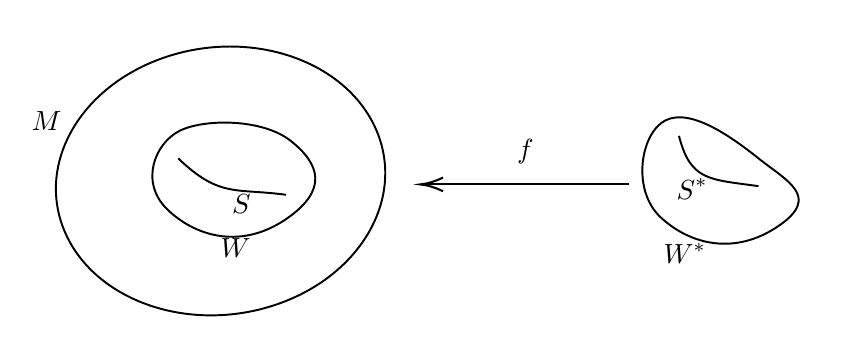
\begin{tikzpicture}[x=0.75pt,y=0.75pt,yscale=-1,xscale=1]
%uncomment if require: \path (0,223); %set diagram left start at 0, and has height of 223

%Shape: Ellipse [id:dp31205351375005885] 
\draw   (35.18,105.18) .. controls (21.37,71.95) and (43.89,34.3) .. (85.46,21.08) .. controls (127.04,7.86) and (171.93,24.08) .. (185.74,57.3) .. controls (199.54,90.53) and (177.03,128.18) .. (135.45,141.4) .. controls (93.87,154.62) and (48.98,138.4) .. (35.18,105.18) -- cycle ;
%Curve Lines [id:da6654336320515477] 
\draw    (90.09,70.38) .. controls (110.06,89.59) and (118.04,84.58) .. (142.01,87.92) ;
%Shape: Polygon Curved [id:ds6403319524310442] 
\draw   (90.89,57.01) .. controls (102.87,51.17) and (130.82,51.17) .. (144.4,62.03) .. controls (157.98,72.89) and (162.77,85.42) .. (142.01,99.62) .. controls (121.24,113.82) and (99.67,108.81) .. (85.3,95.44) .. controls (70.92,82.08) and (78.91,62.86) .. (90.89,57.01) -- cycle ;
%Shape: Polygon Curved [id:ds6985670513888118] 
\draw   (324.92,52) .. controls (336.9,46.15) and (356.07,59.52) .. (369.65,70.38) .. controls (383.23,81.24) and (400,88.76) .. (379.24,102.96) .. controls (358.47,117.16) and (336.9,112.15) .. (322.52,98.78) .. controls (308.15,85.42) and (312.94,57.85) .. (324.92,52) -- cycle ;
%Curve Lines [id:da37504253031609736] 
\draw    (331.31,59.52) .. controls (336.9,81.24) and (345.69,80.4) .. (369.65,83.75) ;
%Straight Lines [id:da1757973560387438] 
\draw    (307.35,82.91) -- (208.71,82.91) ;
\draw [shift={(206.71,82.91)}, rotate = 360] [color={rgb, 255:red, 0; green, 0; blue, 0 }  ][line width=0.75]    (10.93,-3.29) .. controls (6.95,-1.4) and (3.31,-0.3) .. (0,0) .. controls (3.31,0.3) and (6.95,1.4) .. (10.93,3.29)   ;

% Text Node
\draw (109.04,107.33) node [anchor=north west][inner sep=0.75pt]   [align=left] {$\displaystyle W$};
% Text Node
\draw (17.99,46.34) node [anchor=north west][inner sep=0.75pt]   [align=left] {$\displaystyle M$};
% Text Node
\draw (114.54,86.44) node [anchor=north west][inner sep=0.75pt]   [align=left] {$\displaystyle S$};
% Text Node
\draw (322.4,109.67) node [anchor=north west][inner sep=0.75pt]   [align=left] {$\displaystyle W^{*}$};
% Text Node
\draw (328.7,78.76) node [anchor=north west][inner sep=0.75pt]   [align=left] {$\displaystyle S^{*}$};
% Text Node
\draw (251.93,59.71) node [anchor=north west][inner sep=0.75pt]   [align=left] {$\displaystyle f$};


\end{tikzpicture}

    \caption{Surgery}
\end{figure}

\begin{eg}[Hirzebruch]
    Let $M=\mathbb{P}^1\times\mathbb{P}^1$.
    Since $\mathbb{P}^1=\mathbb{C}\cup\{\infty\}$, we can set $S=\{0\}\times\mathbb{P}^1$, $W=\{(z,\zeta)\in\mathbb{C}\times\mathbb{P}^1:\ |z|<\varepsilon\}$ be a neighborhood of $S$ in $M$.
    Let $W^*=\{(z,\zeta)\in\mathbb{C}\times(\mathbb{P}^1)^*:\ |z|<\varepsilon\}$ and $S=\{0\}\times(\mathbb{P}^1)^*$.
    Fix an integer $m>0$ and define $f:W^*\backslash S^*\to W\backslash S$ by
    \[f(z,\zeta^*)=(z,\zeta^*/z^m)\]
    Then $f$ is biholomorphic, let $M_m^*=(M\backslash S)\cup W^*$.
    Hirzebruch proved the following properties in~\cite{Hirzebruch51}:
    \begin{enumerate}
        \item $M$ and $M_m^*$ are topologically different if $m$ is odd.
        \item $M_m^*\not\cong M_n^*$ as complex manifolds when $m\neq n$.
        \item $M^*_{2m}=M$ topologically.
        \item $M^*_{2m+1}=M^*_1$ topologically.
    \end{enumerate}
\end{eg}

\begin{eg}[Blowing up]
    First we discuss the case where $M$ has complex dimension $2$.
    Let $p$ be any point on $M$, $S=\{p\}$ and $S^*=\mathbb{P}^1$.
    We define $M^*=(M\backslash S)\cup\mathbb{P}^1$ as follows:
    Choose a coordinate chart $(W,z)$ such that $z(p)=0$, $|z_1|<\varepsilon,|z_2|<\varepsilon$.
    We define a subvariety $W^*$ of $W\times\mathbb{P}^1$ by
    \[W^*:=\{(z_1,z_2,(\zeta_1,\zeta_2))\in W\times\mathbb{P}^1:\ z_1\zeta_2-z_2\zeta_1=0\}\]
    Since $\partial{f}/\partial{z_1}=\zeta_2,\partial{f}/\partial{z_2}=-\zeta_1$ if $f=z_1\zeta_2-z_2\zeta_1$, $(\partial{f}/\partial{z_1},\partial{f}/\partial{z_2})\neq 0$, hence $W^*$ is a submanifold.
    Let $f^*:W^*\to W$ be the restriction of projection map $W\times\mathbb{P}^1\to W$, then $W^*\supset 0\times\mathbb{P}^1$, $f^*:S^*\to\{p\}$, and $f^*:W^*\backslash S^*\to W\backslash S$ is biholomorphic.
    That is because $f^*$ has inverse $(z_1,z_2)\to(z_1,z_2,(z_1,z_2))$.
    By surgery we obtain $M^*=(M\backslash\{p\})\cup\mathbb{P}^1$.
    We call $M^*$ the \emph{blowing up} of $M$ at $p$, and denote $M^*=\Bl_p(M)$.

    Blowing up can be complicated, a well-known fact in algebraic geometry is for six points $P_1,\cdots,P_6$ in ``general position'' (specified, no three points are colinear and no six points are on a conic), we have
    \[\Bl_{P_6}\cdots\Bl_{P_1}(\mathbb{P}^2)\cong\{\zeta\in\mathbb{P}^3:\ \zeta_0^3+\zeta_1^3+\zeta_2^3+\zeta_3^3=0\}\subset\mathbb{P}^3\]

    General case is similar, if $\dim_\mathbb{C}M=n$, let $p\in M$ and $(W,z)$ be a coordinate chart as above.
    Define the submanifold $W^*:=\{(z,\zeta):\ z_i\zeta_j-z_j\zeta_i=0,\ 1\leq i<j\leq n\}$, and $f^*$ be the restriction of projection map $W\times\mathbb{P}^1\to W$.
    $f^*:(W^*\backslash\mathbb{P}^1)\to(W\backslash\{p\})$ is biholomorphic, so by surgery, we get $\Bl_p(M)=(M\backslash\{p\})\cup\mathbb{P}^1$.
\end{eg}
\chapter{Sheaves and Cohomology}

\section{Algebra Preliminaries}

We first provide some necessary background material on algebra.
All the rings in this chapter will be assumed to be commutative and with unit.

\subsection*{Cochain Complex and Cohomology}

\begin{defn}
    A \emph{cochain complex} $C$ is a graded $R$-module $C=\bigoplus_{n\in\mathbb{N}}C^n$ with homomorphisms
    \[0\to C^0\xrightarrow{\delta^0}C^1\xrightarrow{\delta^1}\cdots\xrightarrow{\delta^{n-1}}C^n\xrightarrow{\delta^n}\cdots\]
    which satisfy $\delta^{n+1}\circ\delta^n=0$ for $n\geq 0$.
    A cochain map between chain complex is a graded homomorphism $f:C\to D$ of degree $0$, making the following diagram commute:
    \[\begin{tikzcd}
        0 \ar[r] & C^0 \ar[d, "f_0"] \ar[r,"\delta^0"] & C^1 \ar[d, "f_1"] \ar[r,"\delta^1"] & \cdots \ar[r,"\delta^{n-1}"] & C^n \ar[d, "f_n"] \ar[r,"\delta^n"] & \cdots \\
        0 \ar[r] & D^0 \ar[r,"d^0"] & D^1 \ar[r,"d^1"] & \cdots \ar[r, "d^{n-1}"] & D^n \ar[r, "d^n"] & \cdots
    \end{tikzcd}\]
\end{defn}

\begin{defn}
    The $i$th \emph{cohomology module} is defined by
    \[H^i(C)=\frac{\ker\delta^i}{\im\delta^{i-1}}\]
    and the cohomology module is defined by the graded module $H^\bullet(C)=\bigoplus_{n\in\mathbb{N}}H^n(C)$.
    A cochain map $f:C\to D$ induces a graded homomorphism $f^*:H^\bullet(C)\to H^\bullet(D)$ of degree $0$, i.e.\ for each $f_i:C^i\to D^i$, $f_i$ induces a homomorphism $f^*_i:H^i(C)\to H^i(D)$.
\end{defn}

We are now going to proof the following theorem:
\begin{thm}[Zig-zag lemma]
    If the sequence of cochain complex
    \[0\to C\xrightarrow{f} D\xrightarrow{g} E\to 0\]
    is exact, then the long sequence of cohomology modules
    \[\begin{tikzcd}
        0 \ar[r] & H^0(C) \ar[r, "f_0^*"] & H^0(D) \ar[r, "g_0^*"] & H^0(E) \ar[dll, "\delta^*"] \\[3mm]
        {} & H^1(C) \ar[r, "f_1^*"] & H^1(D) \ar[r, "g_1^*"] & H^1(E) \ar[dll, "\delta^*"] \\[3mm]
        {} & \cdots & {} & {}
    \end{tikzcd}\]
    is exact.
\end{thm}

For this, we need the following lemmas.

\begin{lem}\label{coho short exact}
    Let $C$ be a cochain complex, the following sequence is exact for $n\geq 0$
    \[0\to\ H^n(C)\to\coker(\delta^{n-1})\xrightarrow{\delta^n}\ker(\delta^{n+1})\to H^{n+1}(C)\to 0\]
\end{lem}
\begin{proof}
    Clearly $\varphi^n:=\delta^n|_{\coker(\delta^{n-1})}$ is well-defined and $\ker(\varphi^n)=H^n(C),\coker(\varphi^n)=H^{n+1}(C)$.
\end{proof}

\begin{lem}[Snake lemma]
    Consider the following commutative diagram with exact rows:
    \[\begin{tikzcd}
        {} & X \ar[r, "f"] \ar[d,"\alpha"] & Y \ar[r, "g"] \ar[d,"\beta"] & Z \ar[r] \ar[d,"\gamma"] & 0 \\
        0 \ar[r] & U \ar[r, "f'"] & V \ar[r, "g'"] & W & {}
    \end{tikzcd}\]
    Then there exists a homomorphism $\delta:\ker(\gamma)\to\coker(\alpha)$ giving rise the following exact sequence
    \[\ker(\alpha)\to\ker(\beta)\to\ker(\gamma)\xrightarrow{\delta}\coker(\alpha)\to\coker(\beta)\to\coker(\gamma)\]
\end{lem}
\begin{proof}
    $\ker(\alpha)\to\ker(\beta)\to\ker(\gamma)$ is exact.
    Let $y\in\ker(g|_{\ker(\beta)})$, then $g(y)=0$, there exists an $x\in X$ such that $f(x)=y$.
    We must show $x\in\ker(\alpha)$.
    We have $0=\beta(y)=\beta(f(x))=f'(\alpha(x))$, and since $f'$ is injective, $\alpha(x)=0$, i.e.\ $x\in\ker(\alpha)$.
    Similarly $\coker(\alpha)\to\coker(\beta)\to\coker(\gamma)$ is exact.

    We now construct a $\delta$ making the sequence exact.
    Take $z\in\ker(\gamma)$, choose $y$ such that $g(y)=z$, then $g'(\beta(y))=\gamma(g(y))=\gamma(z)=0$, hence there exists a unique $u\in U$ such that $f'(u)=\beta(y)$.
    Set $\delta(z)=u+\im(\alpha)$.
    We show $\delta$ is well-defined.
    If $g(y')=z$, let $f'(u')=\beta(y')$, then $g(y-y')=0$, there exists an $x\in X$ such that $f(x)=y'-y$.
    Therefore
    \[f(u'-u)=\beta(y'-y)=\beta(f(x))=f'(\alpha(x))\]
    Since $f'$ in injective, we have $u'-u=\alpha(x)\in\im(\alpha)$, hence $\delta$ is well-defined.
    Consider $\ker(\beta)\to\ker(\gamma)\xrightarrow{\delta}\coker(\alpha)$, let $z\in\ker(\gamma)$ and $\delta(z)=0$.
    Then let $g(y)=z,f'(u)=\beta(y)$, we have $u\in\im(\alpha)$.
    Let $\alpha(x)=u$, then $\beta(y)=f'(\alpha(x))=\beta(f(x))$, we have $y-f(x)\in\ker(\beta)$.
    Moreover, $g(y-f(x))=z$, we have $\ker(\delta)\subset\im(g|_{\ker\beta})$, the sequence is exact.
    Similarly $\ker(\gamma)\xrightarrow{\delta}\coker(\alpha)\to\coker(\beta)$ is exact.
\end{proof}

\begin{proof}[Proof of Zig-zag lemma]
    Consider the following commutative diagram
    \[\begin{tikzcd}
        {} & 0 \ar[d] & 0 \ar[d] & 0 \ar[d] & {}\\
        {} & H^n(C) \ar[d] & H^n(D) \ar[d] & H^n(E) \ar[d] & {}\\
        {} & \coker(\delta^{n-1}_C) \ar[r, "f"] \ar[d] & \coker(\delta^{n-1}_D) \ar[r, "g"] \ar[d] & \coker(\delta^{n-1}_E) \ar[r] \ar[d] & 0 \\
        0 \ar[r] & \ker(\delta^n_C) \ar[r, "f"] \ar[d] & \ker(\delta^n_D) \ar[r, "g"] \ar[d] & \ker(\delta^n_E) \ar[d] & {} \\
        {} & H^{n+1}(C) \ar[d] & H^{n+1}(D) \ar[d] & H^{n+1}(E) \ar[d] & {}\\
        {} & 0 & 0 & 0 & {}
    \end{tikzcd}\]
    Diagram chasing shows the rows are exact, and by Lemma~\ref{coho short exact}, the columns are exact.
    Hence the result follows from Snake lemma.
\end{proof}

Our next result on cohomology is that cohomology is natural.

\begin{thm}[Naturality of cohomology]
    Let
    \[\begin{tikzcd}
        0\ar[r] & C \ar[r]\ar[d, "f"] & D \ar[r]\ar[d, "g"] & E \ar[r]\ar[d, "h"] & 0 \\
        0\ar[r] & C' \ar[r] & D'\ar[r] & E' \ar[r] & 0
    \end{tikzcd}\]
    be commutative diagram of cochain complexes with exact rows, then the long exact sequence of cohomology modules
    \[\begin{tikzcd}
        0 \ar[r] & H^0(C) \ar[r] \ar[d, "f^0"] & H^0(D) \ar[r] \ar[d, "g^0"] & H^0(E) \ar[r, "\delta^*"] \ar[d, "h^0"] & H^1(C) \ar[r] \ar[d, "f^1"] & \cdots\\
        0 \ar[r] & H^0(C') \ar[r] & H^0(D') \ar[r] & H^0(E') \ar[r, "(\delta')^*"] & H^1(C') \ar[r] & \cdots
    \end{tikzcd}\]
    is commute.
\end{thm}
\begin{proof}
    Diagram chasing.
\end{proof}

\subsection*{Direct Limit}

\begin{defn}
    A \emph{direct set} is a preordered set $(I,<)$ such that for $i,j\in I$, there is a $k\in I$ satisfying $i<k,j<k$.
    A \emph{direct system} is a set of rings or $R$-modules indexed by a direct set, with homomorphisms $\varphi_{ij}:M_i\to M_j$ whenever $i<j$ and $\varphi_{jk}\circ\varphi_{ij}=\varphi_{ik}$ whenever $i<j<k$.

    If $\{M_i\}_{i\in I}$ is a direct system, then the \emph{direct limit} of the direct system is a ring or $R$-module $\varinjlim_{i\in I}M_i$ with homomorphisms $\varphi_i:M_i\to\varinjlim_{i\in I}M_i$, satsifying for every $N$ with homomorphisms $\psi_i:M_i\to N$ that compatible with $\varphi_{ij}$'s, then there exists a unique homomorphism $\psi_N:\varinjlim_{i\in I}M_i\to N$ compatible with all homomorphisms.
\end{defn}

We just outline the construction of direct limits.
If $\{M_i\}_{i\in I}$ is a direct system, then $\varinjlim_{i\in I}M_i$ is a quotient of $\coprod_{i\in I}M_i$.
For rings, the coporduct notation stands for disjoint union, and quotient out the following equivalent relation: For $m_i\in M_i,m_j\in M_j$, $m_i\sim m_j$ if there exists $k\in I$ such that $i<k,j<k$ and $\varphi_{ik}(m_i)=\varphi_{jk}(m_j)$;
For $R$-modules, the coproduct notation stands for direct sum, and quotient out the submodule $Q$ generated by elements with form $\iota_i(m_i)-\iota_j(\varphi_{ij}(m_i))$, where $\iota_i$ is the natural embedding. 

\begin{prop}
    If $(I,<)$ is a direct set, $\{M_i'\}_{i\in I},\{M_i\}_{i\in I},\{M_i''\}_{i\in I}$ are direct systems, and for all $i\in I$ the sequence $M_i'\xrightarrow{f_i}M_i\xrightarrow{g_i}M_i''$ is exact, then the sequence
    \[\varinjlim_{i\in I}M_i'\xrightarrow{f}\varinjlim_{i\in I}M_i\xrightarrow{g}\varinjlim_{i\in I}M_i''\]
    is exact.
\end{prop}
\begin{proof}
    We prove for modules.
    Denote $H_i=\ker(g_i)/\im(f_i)$, $H=\ker(g)/\im(f)$.
    Then for each $I$, there is a canonical homomorphism $H_i\to H$.
    This give rise a homomorphism $\varinjlim_{i\in I}H_i\to H$, we need to prove this homomorphism is surjective.
    Let $h\in H$, $h=m+\im(f)$, and let $m=\varphi_i(m_i)$ for some $m_i\in M_i$.
    Then there exists $j\geq i$ such that $\varphi_{ij}''(g_i(m_i))=0$, set $m_j=\varphi_{ij}(m_i)$, then $\varphi_j(m_j)=m$ and $m_j\in\ker(g_j)$.
    Hence the map is surjective.
    But $\varinjlim_{i\in I}H_i=0$, we obtain $H=0$.
\end{proof}

\begin{rem}
    In fact, further argument shows direct limit preserves homology.
    We refer to~\cite[Lemma 10.8.8]{stacks-project}.
\end{rem}

\section{Sheaves}

Instead of using \emph{espace \'{e}tale} as Morrow and Kodaira do, we shall adopt the standard definition of a sheaf.

\begin{defn}
    A \emph{presheaf} $\mathcal{F}$ on a topological space $X$ associates every open set to a group $\mathcal{F}(U)$, called the sections of $\mathcal{F}$ on $U$, and for each two open sets $U\subset V$ there is a \emph{restriction map} $\res^V_U:\mathcal{F}(V)\to\mathcal{F}(U)$ such that:
    \begin{enumerate}[(1)]
        \item For open sets $U\subset V\subset W$, we have $\res^V_U\circ\res^W_V=\res^W_U$;
        \item For open set $U$, we have $\res^U_U=\mathrm{id}_U$.
    \end{enumerate}
    A \emph{sheaf} $\mathcal{F}$ on $X$ is a presheaf satisfying the following two sheaf axioms:
    \begin{enumerate}[(1)]
        \item If for open set $U$ with open cover $U=\bigcup_{i\in I}U_i$ and $f\in\mathcal{F}(U)$, $\res^U_{U_i}f=0,\ \forall i\in I$, then $f=0$;
        \item If for open set $U$ with open cover $U=\bigcup_{i\in I}U_i$, and $f_i\in U_i$ with $\res^{U_i}_{U_i\cap U_j}f_i=\res^{U_j}_{U_i\cap U_j}f_j$, then there exists a unique $f\in U$ such that $\res^U_{U_i}f=f_i$.
    \end{enumerate}
    If the sections are rings, then the sheaf is called a \emph{sheaf of rings}, for $R$-modules \emph{mutatis mutandis}.
\end{defn}

\begin{eg}
    We give some examples of sheaves.
    \begin{enumerate}
        \item Let $M$ be a complex manifold.
        A \emph{holomorphic function} on $M$ is a complex valued function $f$ such that for every atlas $(U,\varphi)$ the function $f\circ\varphi^{-1}$ is holomorphic.
        Define $\mathcal{O}$ as for open set $U$ on $M$, $\mathcal{O}(U)$ is the ring of all holomorphic functions defined on $U$.
        (Notice that any open set on a complex manifold is a complex manifold.)
        \item Let $M$ be a complex manifold.
        Define $\mathcal{O}^*$ satisfy whose sections are nonzero holomorphic functions.
        \item Let $M$ be a complex manifold.
        Define $\mathcal{D}$ satisfy whose sections are differentiable functions.
        \item Let $M$ be a complex manifold.
        Define $\mathbb{Z},\mathbb{R},\mathbb{C}$ to be the sheaf with sections are locally constant $\mathbb{Z}$-, $\mathbb{R}$-, $\mathbb{C}$-valued functions.
    \end{enumerate}
\end{eg}

\begin{defn}
    A \emph{morphism} $f:\mathcal{F}\to\mathcal{G}$ between (pre)sheaves on $X$ is a collection of homomorphisms $f(U)$ for open sets $U$ of $X$, satisfying for any $U\subset V$ the following diagram commutes
    \[\begin{tikzcd}
        \mathcal{F}(V)\ar[r,"f(V)"]\ar[d,"\res^V_U"] & \mathcal{G}(V)\ar[d,"\res^V_U"]\\
        \mathcal{F}(U)\ar[r,"f(U)"] & \mathcal{G}(U)
    \end{tikzcd}\]
    The \emph{kernel} of a sheaf morphism $f:\mathcal{F}\to\mathcal{G}$ is defined as $\ker(f)(U)=\ker(f(U))$.
    To avoid confusion, this means the section of kernel sheaf on $U$ is the kernel of $f(U)$.
    It's easy to verify this is a sheaf.
\end{defn}

\begin{eg}
    We cannot define the image of a morphism in the same way.
    For example, let's take the morphism
    \[\exp:\mathcal{O}\to\mathcal{O}^*\]
    Denote $\preim(\exp)(U)=\im(\exp(U))$, then for every simply connected open set $W\subset\mathbb{C}\backslash\{0\}$, $\mathrm{id}_W\in\preim(\exp)(U)$, but $\mathrm{id}_{\mathbb{C}\backslash\{0\}}\notin\preim(\exp)(\mathbb{C}\backslash\{0\})$, this shows $\preim(\exp)$ does not satisfy the sheaf axiom.
    To fix this, we need the following construction.
\end{eg}

\begin{defn}
    Let $\mathcal{F}$ be a presheaf, then there exists a sheaf $\mathcal{F}^+$ with presheaf morphism $\varphi:\mathcal{F}\to\mathcal{F}^+$, satisfying for any sheaf $\mathcal{G}$ and morphism $f:\mathcal{F}\to\mathcal{G}$, $f$ factors through $\varphi$, i.e.\ there exsits a unique $f^+:\mathcal{F}^+\to\mathcal{G}$ making the following diagram commute
    \[\begin{tikzcd}
        \mathcal{F} \ar[rr, "f"] \ar[dr, "\varphi"] & & \mathcal{G} \\
        {} & \mathcal{F}^+\ar[ur, "f^+"] & {}
    \end{tikzcd}\]
    The sheaf $\mathcal{F}^+$ is called the \emph{sheafification} of $\mathcal{F}$.
\end{defn}

By the definition, sheafification is unique up to an isomorphism (i.e.\ an invertible morphism).
For the construction, we refer to~\cite[Section 6.17]{stacks-project}.

\begin{defn}
    Let $f:\mathcal{F}\to\mathcal{G}$ be a sheaf morphism, and $\preim(f)$ defined as $\preim(f)(U)=\im(f(U))$.
    Then the \emph{image} of $f$ is defined as the sheafification of $\preim(f)$.
\end{defn}

\begin{defn}
    Let $\mathcal{F}\xrightarrow{f}\mathcal{G}\xrightarrow{g}\mathcal{H}$ be sequence of sheaves and morphisms.
    The sequence is called \emph{exact}, if $\im(f)=\ker(g)$.
\end{defn}

\begin{eg}
    The most fundamental exact sequence of sheaves is \emph{exponential sheaf sequence}:
    \[0\to\mathbb{Z}\to\mathcal{O}\xrightarrow{\exp}\mathcal{O}^*\to 0\]
    Where the first morphism is the obvious inclusion, and $\exp(f)=e^{2\pi\sqrt{-1}f}$.
    We check the surjectivity of last morphism.
    Let $f\in\mathcal{O}^*(U)$, then $U$ can be covered by simply connected open sets $\{U_i\}_{i\in I}$ (for instance, open disks).
    On $U_i$ we have $\mathcal{O}^*(U_i)=\im(\exp)(U_i)$, then there is $g_i\in\im(\exp)(U_i)$ such that $g_i=\res^U_{U_i}(f)$.
    By sheaf axiom, there is a unique $g\in\im(\exp)(U)$ such that $\res^U_{U_i}(g)=g_i$ for $i\in I$.
    Mapping $f\mapsto g$, we get a sheaf morphism $\mathcal{O}^*\to\im(\exp)$, then by the uniqueness of sheafification, $\mathcal{O}^*=\im(\exp)$.
\end{eg}

\backmatter

\bibliography{biblio}

\end{document}